\chapter{Giới thiệu}

\ifpdf
\graphicspath{{Chapter1/Chapter1Figs/PNG/}{Chapter1/Chapter1Figs/PDF/}{Chapter1/Chapter1Figs/}}
\else
\graphicspath{{Chapter1/Chapter1Figs/EPS/}{Chapter1/Chapter1Figs/}}
\fi

Những năm gần đây, \textbf{học tăng cường} (reinforcement learning) liên tục đạt được những thành tựu quan trọng trong lĩnh vực Trí tuệ nhân tạo. 
Những đóng góp nổi bật của học tăng cường bao gồm: tự động điều khiển robot di chuyển, điều khiển mô hình máy bay trực thăng, hệ thống chơi cờ vây ... 
Trong số các thành tựu này, hệ thống chơi cờ vây với khả năng chiến thắng những kỳ thủ hàng đầu thế giới là một cột mốc quan trọng của lĩnh vực Trí tuệ nhân tạo. 
Dù vậy, học tăng cường không phải là một phương pháp mới được phát triển gần đây.
Nền tảng lý thuyết của học tăng cường đã được xây dựng từ những năm 1980 \cite{sutton1998introduction}.

Được xây dựng nhằm mô phỏng quá trình học của con người, ý tưởng chính của học tăng cường là tìm cách lựa chọn hành động \textit{tối ưu} để nhận được \textbf{nhiều nhất giá trị điểm thưởng} (reward). 
Giá trị điểm thưởng này có ý nghĩa tương tự cảm nhận của con người về môi trường. 
Khi một đứa trẻ bắt đầu ``học'' về thế giới xung quanh của mình, những cảm giác như đau đớn (ứng với điểm thưởng thấp) hay vui sướng (điểm thưởng cao) chính là mục tiêu cần tối ưu của việc học. 
Việc đứa trẻ thực hiện các hành động để tăng cảm giác vui sướng (và giảm đau đớn) cũng tương đồng với việc hệ thống học tăng cường tối đa hoá giá trị điểm thưởng.
Một điểm quan trọng của học tăng cường là các thuật toán được xây dựng với ít giả định nhất có thể về môi trường xung quanh.
Hệ thống sử dụng học tăng cường (agent) không cần biết cách thức hoạt động của môi trường để hoạt động. 
Ví dụ như để điều khiển robot tìm được đi trong mê cung, hệ thống không cần biết mê cung được xây dựng thế nào hay kích thước là bao nhiêu. 
Việc hạn chế tối đa những ràng buộc về dữ liệu đầu giúp cho thuật toán học tăng cường có thể áp dụng vào nhiều bài toán thực tế.

Học tăng cường được xem là một nhánh trong lĩnh vực máy học ngoài hai nhánh: \textit{học có giám sát} và \textit{học không có giám sát}. 
Trong bài toán học có giám sát, dữ liệu học thường được gán nhãn thủ công sẵn (hand-labeled); hệ thống cần tìm cách mối liên hệ giữa dữ liệu và nhãn tương ứng.
Mối liên hệ tìm được sẽ dùng để dự đoán nhãn của dữ liệu mới.
Các nhãn này có thể xem như là sự hướng dẫn trong quá trình học; tính đúng sai của việc học lúc này có thể được xác định dựa vào kết quả dự đoán của hệ thống và nhãn đúng của dữ liệu. 
Tiếp theo đối với những bài toán học không có giám sát, dữ liệu học thường không được gán nhãn nên công việc của việc học là phải tự tìm ra được cấu trúc ``ẩn'' bên dưới dữ liệu đó. 
Khác với hai loại bài toán vừa nêu, trong bài toán học tăng cường, hệ thống \textit{không nhận được nhãn thực sự} (tức hành động tối ưu của tình huống hiện tại) mà chỉ nhận được điểm thưởng từ môi trường. 
Điểm thưởng lúc này chỉ thể hiện mức độ ``tốt/xấu'' của hành động vừa chọn chứ không nói lên hành động đó có phải là hành động tối ưu hay không. 
Điểm thưởng này thông thường rất \textbf{thưa}: ta có thể chỉ nhận được điểm thưởng có ý nghĩa (khác không) sau hàng trăm hành động. 
Ngoài ra, giá trị điểm thưởng thường không đơn định và rất \textbf{nhiễu}: cùng một hành động tại cùng một trạng thái, ta có thể nhận được điểm thưởng khác nhau vào hai thời điểm khác nhau. 
Hai vấn đề này (tính thưa và nhiễu của điểm thưởng) cũng chính là những khó khăn cơ bản của bài toán học tăng cường.

Các trò chơi điện tử thường hay có điểm số mà người chơi cần phải tối ưu hoá. 
Đặc điểm này trùng với yêu cầu của bài toán học tăng cường, vì vậy các trò chơi này cũng chính là những ứng dụng tự nhiên nhất của phương pháp học tăng cường. 
Trong luận văn này, chúng em áp dụng phương pháp học tăng cường nhằm xây dựng \textbf{hệ thống tự động chơi các game} trên hệ máy Atari. 
Dữ liệu đầu vào của hệ thống chỉ bao gồm các frame ảnh RGB cùng với điểm số. 
Từ hình ảnh thô này, hệ thống cần tìm cách chơi sao cho điểm số cuối màn chơi (episode) là lớn nhất có thể.
Lưu ý rằng điểm số được game cung cấp hệ thống dưới dạng số thực (chứ không cần phải nhìn hình ảnh thô để ``đọc'' điểm số).
Điểm khó khăn của bài toán này là hệ thống hoàn toàn không biết quy luật của game trước khi bắt đầu quá trình học mà phải tự tìm hiểu quy luật và chiến thuật chơi tối ưu. 
Lý do luận văn sử dụng game của máy Atari là vì các game này có quy luật chơi tương đối đơn giản nhưng lại rất đa dạng. 
Mỗi màn chơi thường có độ dài vừa phải (từ 2 - 15 phút) và số hành động có ý nghĩa không quá nhiều (18 hành động). 
Ngoài ra, các trò chơi này có thể được giả lập trên máy vi tính với tốc độ cao, giúp quá trình học được tăng tốc.

\begin{figure}
	\centering
	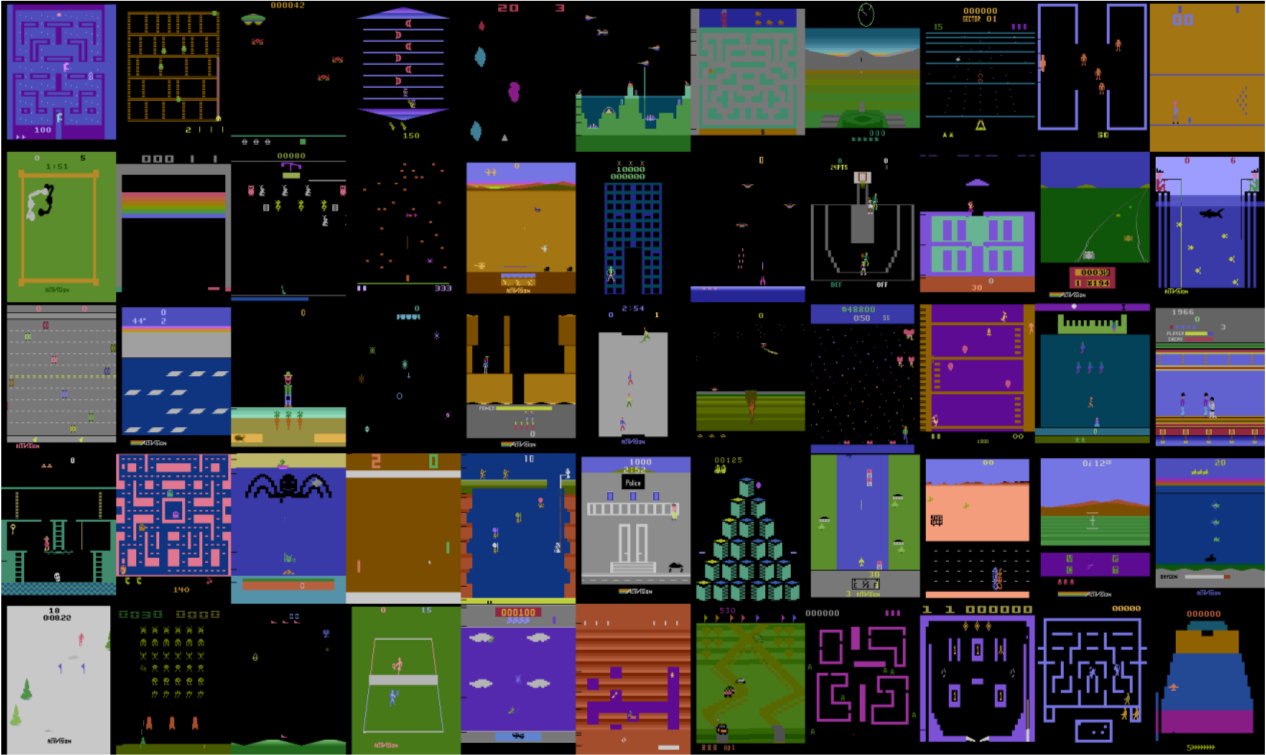
\includegraphics[width=\textwidth]{ale_55_games}
	\caption[Hình ảnh các game trên hệ máy Atari]{Hình ảnh các game trên hệ máy Atari.
	Hình được chỉnh sửa từ \cite{defazio2014comparison}}
	\label{Ale55Games}
\end{figure}

Một số khó khăn trước mắt có thể thấy ở bài toán tự động chơi game bao gồm:
\begin{itemize}
	\item \textbf{Hệ thống biết luật chơi của game}. 
	Chính vì thế nó cũng không thể biết được hành động nào nên làm hoặc không nên làm ứng với từng tình huống cụ thể.
	\item \textbf{Dữ liệu đầu vào là hình ảnh thô} (ảnh RGB có kích thước $210\times160$). 
	Để học được một chiến thuật chơi đơn giản thì hệ thống cũng phải chơi ``thử và sai'' một số lượng lớn màn chơi (có thể lên đến 10000 frame). 
	Vì vậy, lượng dữ liệu đầu vào cần phải xử lý là rất lớn.
	\item \textbf{Các game rất khác nhau}.
	Khác biệt này là về cả hình ảnh lẫn nội dung của game.
	Để có thể học cách chơi của nhiều game khác nhau thì thuật toán học phải mang tính tổng quát cao, không sử dụng các tính chất riêng biệt của từng game.
	\item \textbf{Cần có chiến thuật chơi riêng biệt cho từng game}.
	Để đạt được điểm số cao (ngang hoặc hơn điểm số của con người) thì phải tìm được chiến thuật chơi mang tính lâu dài. 
	Những phương pháp tham lam, lựa chọn hành động để đạt điểm tối đa trong tương lai gần thường không tối ưu.
\end{itemize}

%[TODO: Thêm hướng tiếp cận liên quan + các thực nghiệm + Reference]

%Nhiều phương pháp đã được đề xuất để giải quyết bài toán tự động chơi những game trên hệ máy Atari 2600. Hướng tiếp cận thông thường thường gồm hai giai đoạn [,]. Giai đoạn đầu rút trích đặc trưng từ những frame đầu vào. Trong giai đoạn này ngoài việc chọn ra những đặc trưng tốt cho việc học, nó cũng giúp giảm kích thước dữ liệu đầu vào cho mô hình học. Giai đoạn sau đó thực hiện xấp xỉ hàm 'đánh giá hành động' với đầu vào là những đặc trưng đã rút trích được trong giai đoạn đầu. Nhược điểm của hướng tiếp cận này là mô hình học phức tạp và khó khăn lựa trọn đặc trưng phù hợp cho nhiều game. 
Một trong những tiếp cận đầu tiên cho bài toán tự động chơi game là cuộc thi AAAI General Game Playing được đề xuất từ năm 2005 bởi đại học Stanford \cite{genesereth2005general}.
Trong cuộc thi này, các đội thi nhận được mô tả sơ bộ cho những game được sử dụng để thi.
Các mô hình chi tiết được thiết kế bên dưới các game này không được mô tả cho các đội chơi.
Dựa vào những thông tin nhận được, các đội chơi phải thiết kế một mô hình tổng quát để có thể chơi những game này; trong cuộc thi, họ sẽ chơi ngẫu nhiên một trong những game đã được mô tả \cite{genesereth2005general}.
Đội thắng cuộc trong cuộc thi này đã sử dụng mô hình ``Monte Carlo Tree Search'' (một mô hình phổ biến của học tăng cường) để tìm chiến lược chơi trong những game này.

Trong khoảng ba năm trở lại, tập những game trên hệ máy Atari 2600 trở nên phổ biến trong việc đánh giá khả năng của những phương pháp tiếp cận cho bài toán tự động chơi game.
Những game này bao gồm nhiều thể loại khác nhau như: đối kháng, chiến thuật...
Sự đa dạng trong cách chơi của những game Atari 2600 cùng giao diện lập trình đơn giản làm cho chúng gây được sự chú ý lớn trong cộng đồng Trí tuệ nhân tạo.
Nhiều phương pháp đã được đề xuất liên quan tới bài toán tự động chơi game trên hệ máy Atari 2600. \cite{bellemare2013bayesian,icml2014c2_bellemare14} thực hiện chia những frame ảnh trong game thành nhiều phần; sau đó xây dựng cấu trúc cây  và áp dụng mô hình học Bayesian để mô phỏng lại mô hình của "môi trường" đã được xây dựng trong các game này cho hệ thống.
Tuy nhiên, hướng tiếp cận này giả định những phần ảnh lân cận là đủ thông tin để dự đoán những phần ảnh trung tâm, do đó không phù hợp trong một vài game Atari có sự tương tác phức tạp.
\cite{hausknecht2014neuroevolution} sử dụng mạng nơ-ron với cấu trúc nông để tạo ra một chính sách có thể tự động chơi một số game Atari.
Phương pháp sử dụng thuật toán lập trình tiến hóa để tìm trọng số liên kết tối ưu trong mạng nơ-ron, khác với phương pháp truyền thống sử dụng lan truyền ngược.
Mặc dù phương pháp này vượt qua điểm số của con người trong ba game Atari nhưng còn nhiều hạn chế.
Một trong những hạn chế đó là đặc tính của lập trình tiến hóa hoạt động giống như một ``hộp đen'', nghĩa là chúng ta không thể dễ dàng quan sát, cũng như kiểm soát cách tìm kiếm những trọng số của mạng nơ-ron như đã làm với lan truyền ngược \cite{risi2014neuroevolution}.

Trong những năm gần đây, học sâu đạt đươc nhiều bước đột phá trong nhiều lĩnh vực như Thị giác máy tính, Nhận diện giọng nói...  
Việc kết hợp học tăng cường với học sâu đã dẫn đến một hướng tiếp cận mới cho bài toán tự động chơi game; hướng tiếp cận này giúp hệ thống có thể học cách chơi nhiều game khác nhau từ hình ảnh đầu vào RGB \cite{mnihdqn2015}. 
Với học sâu, ta có thể học được những đặc trưng cấp cao (high level features) từ hình ảnh thô mà không cần phải tự thiết kế đặc trưng bằng tay (hand-designed features). 
Khi kết hợp với học tăng cường, ta có một hình ``\textbf{End-to-end}'': việc học đặc trưng và học chiến thuật chơi được liên kết chặt chẽ với nhau. 
Trong luận văn này, chúng em thực hiện việc cài đặt lại phương pháp học tăng cường sâu và thử nghiệm mô hình với những tham số khác nhau. 
Cùng với đó, luận văn tìm hiểu những khó khăn cơ bản của bài toán tự động chơi game cũng như thử nghiệm lại các đề xuất nhằm giải quyết những khó khăn này.